\subsection{FEABench (Finite Element Analysis Benchmark): Evaluating Language Models on Multiphysics Reasoning Ability}
{{\footnotesize
\noindent N/A


\begin{description}[labelwidth=4cm, labelsep=1em, leftmargin=4cm, itemsep=0.1em, parsep=0em]
  \item[date:] 2023-01-26
  \item[version:] 1
  \item[last\_updated:] 2023-01-26
  \item[expired:] false
  \item[valid:] no
  \item[valid\_date:] 2023-01-26
  \item[url:] \href{https://github.com/google/feabench}{https://github.com/google/feabench}
  \item[doi:] unknown
  \item[domain:]
    - Mathematics
  \item[focus:] FEA simulation accuracy and performance
  \item[keywords:]
    - finite element
    - simulation
    - PDE
  \item[licensing:] unknown
  \item[task\_types:]
    - Simulation
    - Performance evaluation
  \item[ai\_capability\_measured:]
    - Numerical simulation accuracy and efficiency
  \item[metrics:]
    - Solve time
    - Error norm
  \item[models:]
    - FEniCS
    - deal.II
  \item[ml\_motif:]
    - Reasoning \& Generalization
  \item[type:] Benchmark
  \item[ml\_task:]
    - Supervised Learning
  \item[solutions:] unknown
  \item[notes:] OK
  \item[contact.name:] unknown
  \item[contact.email:] unknown
  \item[datasets.links.name:] FEABench Github
  \item[datasets.links.url:] \href{https://github.com/google/feabench?tab=readme-ov-file\#datasets}{https://github.com/google/feabench?tab=readme-ov-file\#datasets}
  \item[results.links.name:] unknown
  \item[results.links.url:] \href{unknown}{unknown}
  \item[fair.reproducible:] Yes
  \item[fair.benchmark\_ready:] Yes
  \item[id:] feabench\_finite\_element\_analysis\_benchmark\_evaluating\_language\_models\_on\_multiphysics\_reasoning\_ability
  \item[Citations:] \cite{mudur2025feabenchevaluatinglanguagemodels}
\end{description}

{\bf Ratings:} ~ \\

\begin{tabular}{p{0.15\textwidth} p{0.07\textwidth} p{0.7\textwidth}}
\hline
Rating & Value & Reason \\
\hline
dataset & 4 & Available, but not split into sets
 \\
documentation & 5 & In associated paper
 \\
metrics & 5 & Fully defined metrics
 \\
reference\_solution & 4 & Three open-source models were used. No system constraints.
 \\
software & 4 & Code is available, but poorly documented
 \\
specification & 1 & Output is defined and task clarity is questionable
 \\
\hline
\end{tabular}

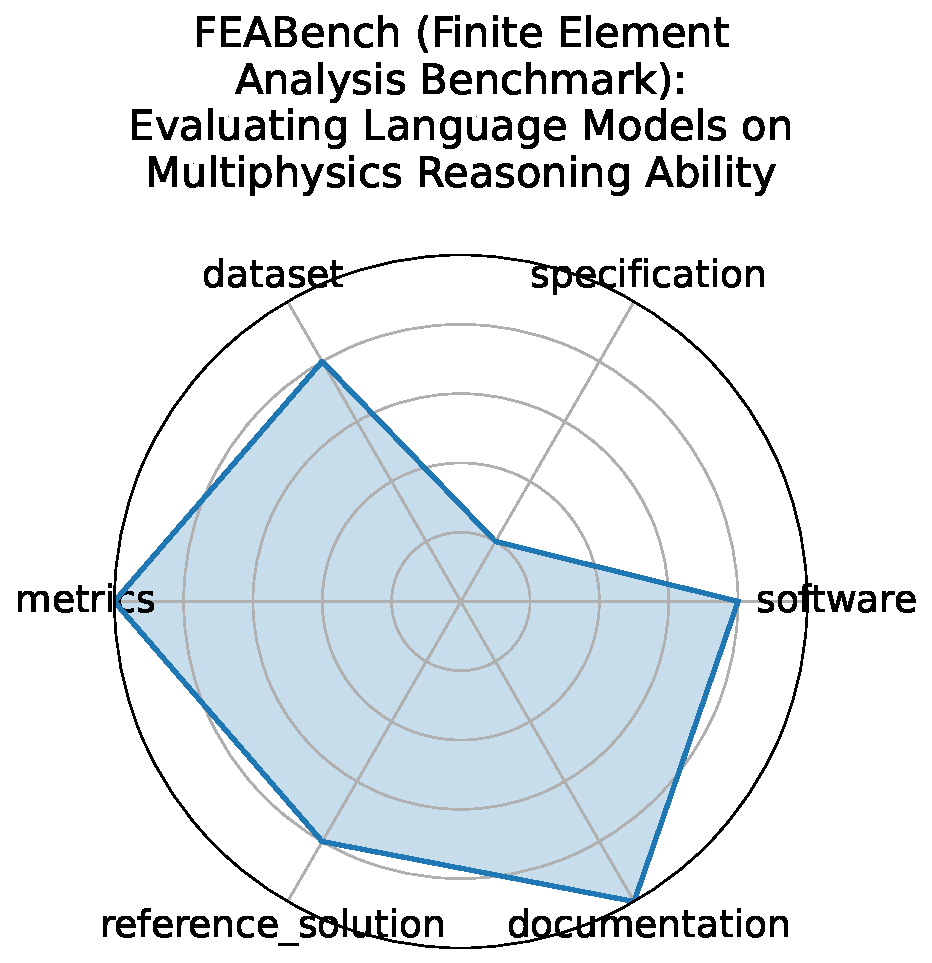
\includegraphics[width=0.2\textwidth]{feabench_finite_element_analysis_benchmark_evaluating_language_models_on_multiphysics_reasoning_ability_radar.pdf}
}}
\clearpage